\documentclass{article}
%\usepackage{fullpage}
\usepackage{fancyhdr}
\usepackage[english,francais]{babel}
\usepackage[T1]{fontenc}
\usepackage[utf8]{inputenc}
\usepackage[pdftex]{graphicx}
\usepackage{subfig}

%\renewcommand{\baselinestretch}{2}
\author{Florent \textsc{Guiotte} et Frédéric \textsc{Becker}}
\title{Seam Carving}
\pagestyle{fancy}

\begin{document}
\maketitle
\tableofcontents

\section{Introduction}

Le seam carving est un algorithme de redimensionnement d'image qui permet de garder intact les éléments <<importants>>
de l'image. Cet algorithme utilise une fonction d'énergie (gradient dans notre cas) pour détecter les zones d'intérêts
de l'image.

Dans la première partie de ce TP nous avons travaillé sur l'image verticale 
représentant un loup et la pleine lune (figure \ref{fig:loup}  à la page \pageref{fig:loup}).
Le but de l'algorithme est de rapprocher la lune du loup sans les déformer en réduisant la hauteur de l'image.

\begin{figure}[!ht]%htp]
  \centering
  \subfloat[Image d'origine]{\label{fig:loup}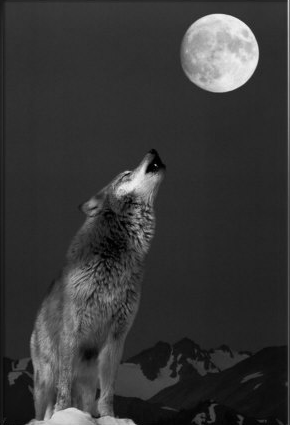
\includegraphics[width=0.48\textwidth]{img/loup.png}}
  \hspace{0.030\textwidth}
  \subfloat[Gradient de l'image]{\label{fig:gradient}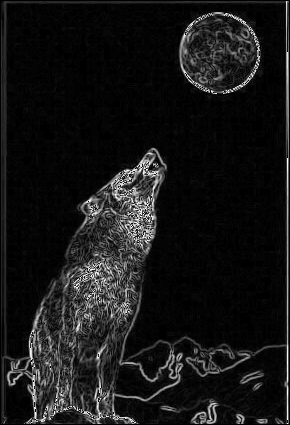
\includegraphics[width=0.48\textwidth]{img/energie.png}}
  \caption{Loup.pgm et calcul de l'énergie associée}
  \label{fig:init}
\end{figure}



\section{Réalisations}
\subsection{Fonction d'énergie}
Pour déterminer l'énergie des pixels de l'image nous avons utilisé la mesure du gradient de l'image. Les pixels se
trouvant dans les zones de gradient faible seront éliminés les premiers.

Notre implémentation du calcul de gradient est visible figure \ref{fig:gradient}. On distingue bien les éléments que l'on veut garder de l'image d'origine. L'utilisation du gradient est plutôt efficace dans le cas de cette image.

\subsection{Chemin minimum}
Dans l'algorithme du seam carving, pour réduire la hauteur de l'image d'un pixel, il faut enlever la <<couture>>
horizontale d'énergie minimale.
Pour  déterminer la couture ayant l'énergie la plus faible dans l'image, on utilise l'algorithme de \textsc{Viterbi}.

\begin{figure}[!ht]
    \center
    \label{seams}
    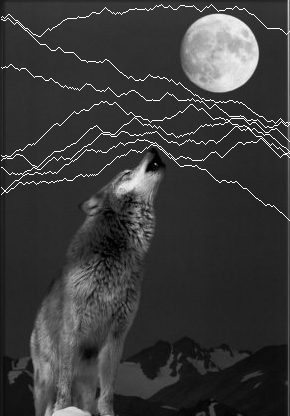
\includegraphics[width=0.48\textwidth]{img/seams.png}
    \caption{Coutures d'énergie minimale}
\end{figure}



\end{document}
